\section{Text Regression in Legal Judgments}\label{sec:text_regression}

The experiments, results and discussions presented in this section are related to text regression. Firstly, there are the experiment's purposes, and how they help on answering the research question. Then, it presents the details on the datasets, pipeline, the results, and the discussion.\footnote{The code is available at \url{https://github.com/thiagordp/text_regression_in_law_judgments}.}


\subsection{Experiment's purpose}

% Entregar um resultado útil para o judiciário.

The experiment's purpose is to answer the third part of the research question, i.e., to what extent the prediction of compensation values can be \emph{accurate} and \emph{helpful} in the legal environment using regression models, we set up pipelines for text regression which include some TM and ML techniques. We start from a simple pipeline, called \emph{baseline}. Then, it receives several improvements, or \emph{adjustments}, forming a new pipeline, called \emph{full pipeline}.

% Based on the results achieved by the pipelines, the legal expert evaluates whether they are helpful in the context of compensation for immaterial damage for legal cases from \gls{JEC}.
% In the case of legally acceptable results, they may be applied in the conciliation hearing at \gls{JEC} and help the parts to have a deal, excluding the necessity of waiting to the final judgment and speed up the cases solution.

To setup the experiments and the pipelines, we used the Python programming language combined with the Scikit Learn~\cite{Pedregosa2012} version 0.24.1, the \gls{NLTK}~\cite{Loper02}, the Pandas library, version 1.2.3~\cite{Mckinney2010}, and Matplotlib, version 3.3.4~\cite{Hunter:2007}.

\subsection{Dataset}\label{sec:regression_dataset}

The dataset is similar to those presented in Section \ref{sec:text_representation} and Section \ref{sec:text_classification}. It is composed of 940 legal judgments issued between February 2011 to September 2020 into the \gls{JEC} located at the \gls{UFSC}. 


The dataset contains a vocabulary of 16,924 words, 712,057 total tokens and an average of 758 tokens per document (after the preprocessing step). The labels (compensation values) vary from 304 to 25,000 Brazilian \textit{Reais} with an average of 6,344 and a standard deviation of 3,471. In other words, only judgments with \textit{well founded} or \textit{partly well founded} results may appear in this dataset as they have compensation values bigger than zero.


Similar to the text representation and text classification experiments, to evaluate the model, we remove the part of the document that refers to the result of the judgment since it contains the value of compensation for immaterial damage. That way, the models predicts the compensation value based on the report and the legal reasons for the decision. 
The result part is only used to set the legal cases' labels. 


As a complement to the textual dataset, a legal expert manually extracted some attributes and their values from each document, which was possible through a clustering step. 
One of the attributes identified, for example, is the flight delay period. Therefore, the expert analyzed every judgment and extracted the value of this attribute (the delay hours).

It follows the list of such attributes together with an explanation of their importance for the prediction problem.

\begin{itemize}[topsep=1em,leftmargin=1.5\parindent,align=left,labelwidth=0.5\parindent, noitemsep]
  \item \textbf{Date of judgment:} The judge's perspectives may change over time. Consequently, the amount of compensation may vary by date. In the dataset, this is represented by day, month, and year.
  \item \textbf{Judge:} Each judge is free to set the amount of compensation according to his/her conviction on the case. In this sample period, the judgments were elaborated by different judges. In the dataset, this is represented by the name of the thirty one judges who prepared the collected judgments.
  \item \textbf{Type of judge:} In the \gls{JEC}, there are three types of judges: chief, assistant, and voluntary. The chief judge is responsible for the court and is the one who, as a rule, judges the lawsuits. The assistant or substitute judge is the one who judges when the chief judge needs to be absent. And the voluntary judge is the one who has a law degree but is not invested in the position. He or she voluntarily prepares judgments that are submitted to the approval of the chief judge. An assistant judge can freely fix a different value of compensation than a chief judge. The voluntary judge can do this too, but the chief judge can modify the value. In the dataset, this is represented by the a categorical variable. 
  \item \textbf{Permanent baggage loss:} It is an event that can generate compensation for immaterial damage. In the dataset, this is represented by ``yes'' (when there was a loss) and ``no'' (when there was no loss).
  \item \textbf{Tampered baggage:} Depending on the level of damage or in case of missing consumer's belongings (theft), it is an event that can generate compensation for immaterial damage. In the dataset, this is represented by ``yes'' (when there was tampering) and ``no'' (when there was no tampering). 
  \item\textbf{Temporary baggage loss:} It is an event that can generate compensation for immaterial damage. In the dataset, this is represented by ``yes'' (when there was a loss) and ``no'' (when there was no loss).
  \begin{itemize}[noitemsep]
    \item \textbf{Loss interval: }It is a sub-attribute. The longer the delay in returning the baggage to the consumer, the greater can be the value of the compensation for immaterial damage. In the dataset, this is represented by days.
  \end{itemize}
  \item \textbf{Flight cancellation:} It is an event that can generate compensation for immaterial damage. We consider as flight cancellation those cases with no rebooking or when the destination is changed. In the dataset, this is represented by ``yes'' (when there was cancellation) and ``no'' (when there was no cancellation).
  \item \textbf{Flight delay:} It is an event that can generate compensation for immaterial damage. We consider as flight delay those cases with rebooking. In the dataset, this is represented by ``yes'' (when there was a delay) and ``no'' (when there was no delay).
  \begin{itemize}[noitemsep]
    \item   \textbf{Delay interval: }It is a sub-attribute. The longer the delay in rebooking (that is, the longer the interval between the initially contracted flight and the actual flight operated), the greater can be the value of the compensation for immaterial damage. In the dataset, this is represented by hours and minutes.
   \end{itemize}
   \item \textbf{Adverse weather conditions:} It is an event that excludes the possibility of compensation for immaterial damage because it is an unpredictable situation. Even the airline effort is not capable of overcoming them, so there is no way to impute liability to it. In the dataset, this is represented by ``yes'' (when there was proven bad weather) and ``no'' (when there was no proven bad weather). 
   \item \textbf{Consumer fault:} It is an event that excludes the possibility of compensation for immaterial damage because it removes the airline's liability. An example of this situation is when the consumer does not arrive at the airport in plenty of time to check his/her flight and bags. In the dataset, this is represented by ``yes'' (when there was the consumer fault) and ``no'' (when there was no consumer fault).
   \item\textbf{Overbooking:} Selling more tickets for a flight than are available is considered an abusive practice. Thus, it is an event that can generate compensation for immaterial damage. In the dataset, this is represented by ``yes'' (when there was overbooking) and ``no'' (when there was no overbooking). 
   \item\textbf{No show:} Cancellation of the return ticket unilaterally when the consumer does not show up on the outward flight is considered an abusive practice. Thus, it is an event that can generate compensation for immaterial damage. In the dataset, this is represented by ``yes'' (when there was cancellation by no show) and ``no'' (when there was no cancellation by no show).
   \item \textbf{Right to regret and repayment claim:} Hindering the consumer's repayment when he/she decides to cancel the acquired ticket is an event that can generate compensation for immaterial damage. This situation is known by a sequence of bad experiences (called \textit{via crucis} by judges) that the consumer must face getting the repayment. In the dataset, this is represented by ``yes'' (when repayment was hindered) and ``no'' (when the repayment was not hindered or when there was no claim).
  \item \textbf{Downgrade:} The airline changes a business class passenger to economy class. Besides a breach of contract, it is also a breach of the consumer's expectation, and, therefore, it is an event that can generate compensation for immaterial damage. In the dataset, this is represented by ``yes'' (when there was a downgrade) and 
  ``no'' (when there was no downgrade).
\end{itemize}



\subsection{Pipeline}\label{sec:regression_pipeline}

To answer the research question, we propose the application of several TM and ML techniques on a pipeline for regression on legal texts.
% Apresentar a Figura do Pipeline
Thereby, we aim to create learning models capable of making accurate and helpful predictions for immaterial damage compensation. Figure~\ref{fig:pipeline} shows the proposed pipeline, built upon the one from Section~\ref{sec:back_regression}. 
We incremented it with \gls{TM} and \gls{ML} techniques, called \textit{adjustments}.

\begin{figure}[htb]
  \caption{Full pipeline for legal text regression}
  \label{fig:pipeline}
  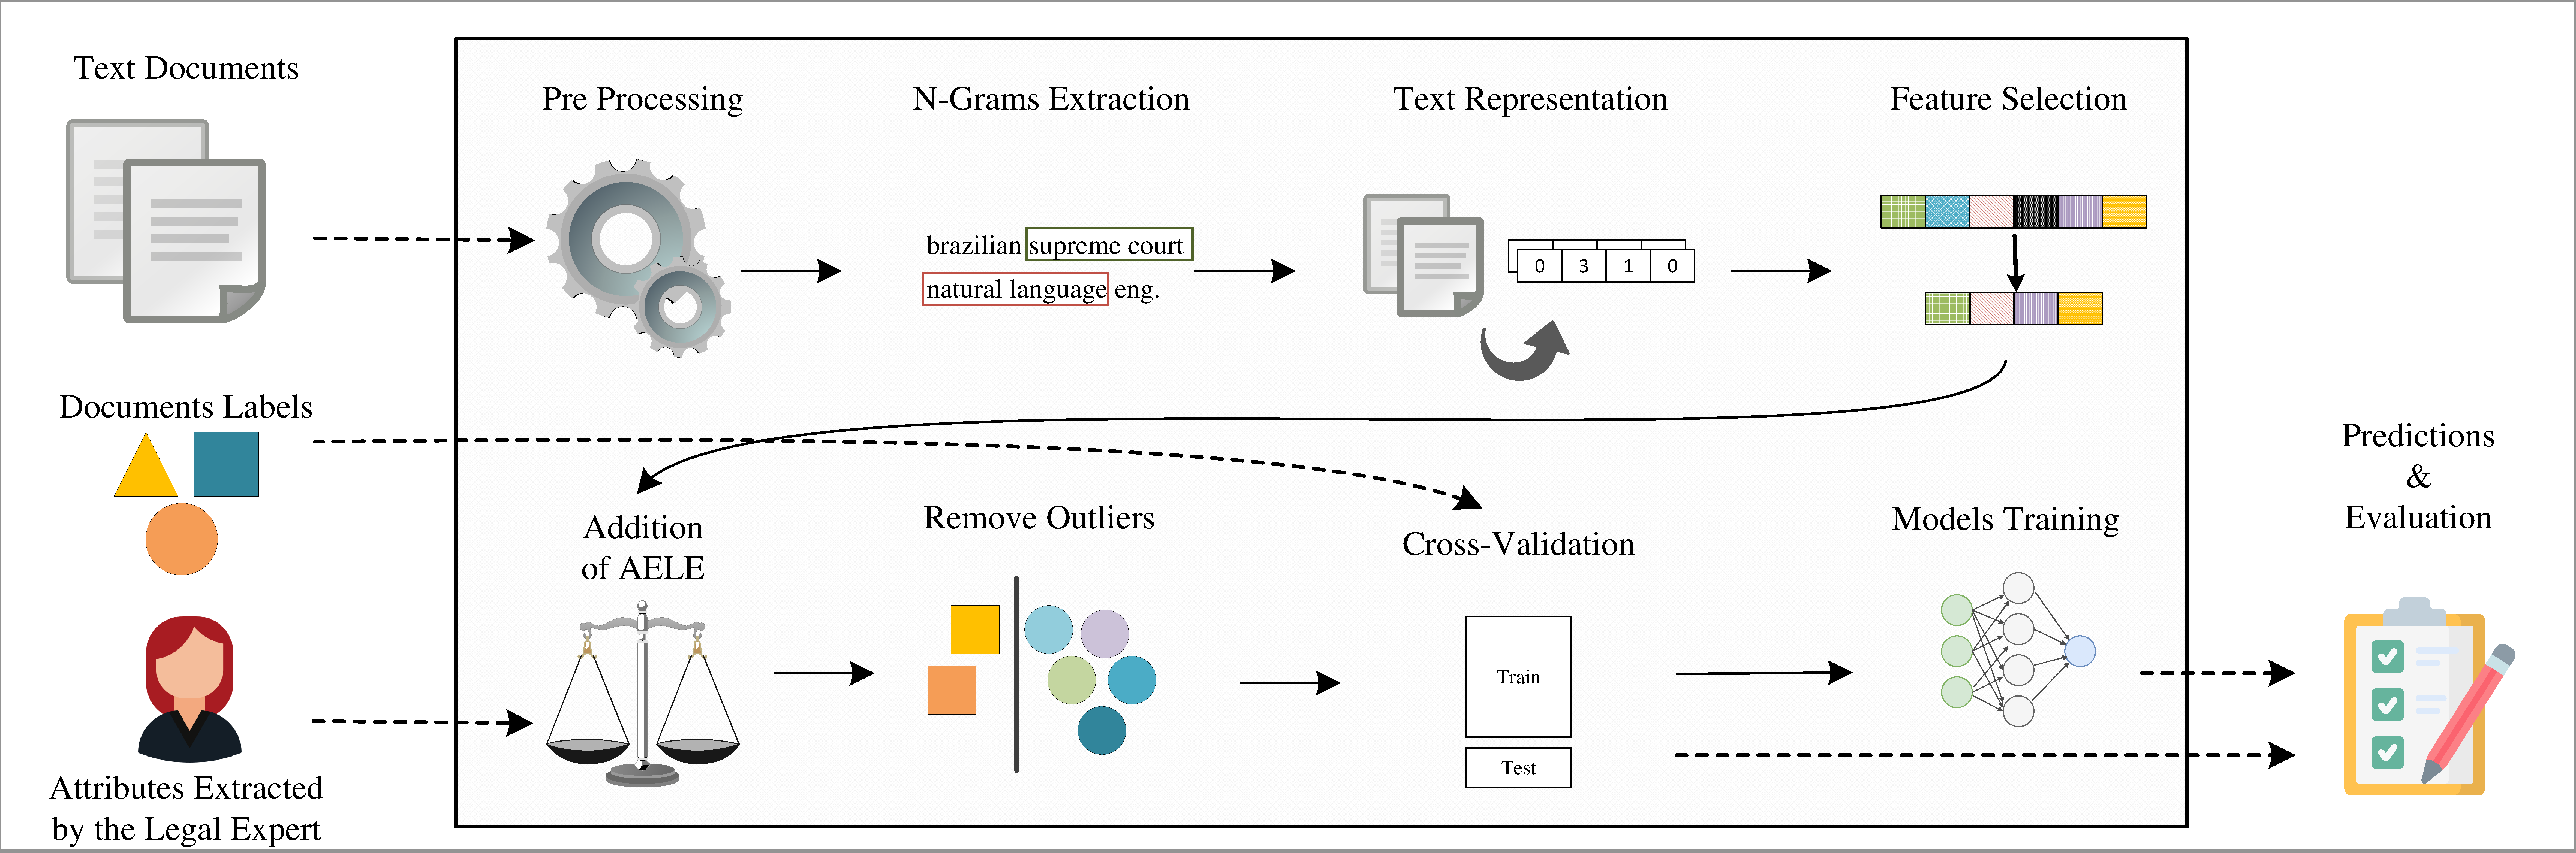
\includegraphics[width=\textwidth]{images/chapters/proposed_pipeline_v3.pdf}
\end{figure}


% Explicar o passo a passo e as ferramentas utilizadas.
The pipeline receives three types of input: the text of the legal judgments, their labels, and the \gls{AELE} for each document (cf. Section~\ref{sec:regression_dataset}).
The preprocessing step converts the text to lowercase and remove noise characters, punctuation, stopwords such as \textit{de}, \textit{para} (prepositions in Portuguese), using the \gls{NLTK}~\cite{bird:2004}.

The first adjustment is \emph{N-Grams Extraction}, varying in length from one to four. However, as this range would lead to an unreasonable dimensionality, we limited the BOW representation to the 25,000 most frequent units, using Scikit-Learn~\cite{Pedregosa2012}.


For the text representation, we use \gls{BOW} using \gls{TF} values. We also tested word embeddings trained with legal documents written in Portuguese and \gls{TF} combined with \gls{IDF}, although TF achieved the best results for the experiments presented in this work. 


The second adjustment is \emph{Feature Selection}, using the Mutual Information method. It maps the relationship between each feature (unit in the BOW) and the dependent variable~\cite{Cover2005}, the amount of immaterial damage compensation. As we tested a wide range of values as the number of features to select, we set it to 500 to consume less time on the experiments and still achieve good results.

The third adjustment is \emph{Addition of \gls{AELE}}, based on the attributes described in Section~\ref{sec:regression_dataset}. Categorical features such as \textit{judges} and \textit{types of judges} were converted to one-hot encoding. Real value features, such as \textit{delay interval}, were not modified. 
In the end, the final representations of the documents were composed of a concatenation of the 52 features from the legal attributes and the \gls{BOW} features. In the case when feature selection is activated, there were 500 \gls{BOW} features. Otherwise, there were 50,000 (the reasons to activate or not an adjustment are detailed later in this section).
% In the end, the final representations of the documents were composed of 52 features from the legal attributes and the \gls{BOW} features. That is, 500 when feature selection is activated or 50,000, otherwise (the reasons to activate or not an adjustment are detailed later in this section).

% Remove Outliers
The fourth adjustment is \emph{Outliers Removal}. As previously described, outliers are very distinctive examples in the dataset, and by removing them, we make it easier for the models to learn. To detect outliers, we used the Isolation Forest with contamination set to ten per cent. Moreover, we have placed this step in two different positions: before and after cross-validation, but we did not apply both in the same pipeline. The former intends to remove outliers from the whole dataset, while the latter, from the train set. By removing outliers from all dataset, we imply that our future cases for prediction will not contain outliers. 


% Cross Validation
The fifth adjustment is \emph{Cross-Validation}, which uses multiple combinations of the train and test sets and the resulting metrics are averaged. In this work, we set the number of folds to five, so, in each step, eighty per cent and twenty per cent of the dataset is used for train and test, respectively.

% Models Trainig
The selected techniques of ML for the regression task are listed in Table~\ref{tab:models}. We used the AdaBoost (AB), Bagging (BG), Decision Trees (DT), feed-foward Neural Networks (NN), \gls{EN}, \gls{EV}, Gradient Boosting (GB), Random Forest (RF), \gls{RG}, Support Vector Machine (SVM), and XGBoosting (XGB). 

Considering the problem of overfitting, we evaluate them for two configurations: \textit{simple} and \textit{complex}. In the former, we define some constraints to the models such as the number of iterations and maximum tree levels, while in the latter we let the models free, without such constraints. The forth column of the table contains the parameter values used in both configurations and any unlisted parameters in Table~\ref{tab:models} follow the default values from Scikit-Learn~\cite{Pedregosa2012}. 

Finally, the sixth adjustment is \emph{Overfitting Avoidance}, that is implemented by simpler models in our pipeline. And, we note that Ensemble Voting Model is an ensemble of ensembles, so it uses models like Bagging and XGBoosting with the same parameters as described in their respective lines.


\begin{table}[htb]
\centering
  \setlength{\tabcolsep}{0pt}
 \caption{Regression techniques and parameters}
 \label{tab:models}

\footnotesize
\begin{tabular}{@{}cccc@{}}
\toprule
\textbf{Technique}   & \textbf{Parameters (Complex)}                                                         & \textbf{Parameters (Simple)}                                                         & \textbf{Common Parameters}                         \\ \midrule
AB      & Nº Estimators: 100                                                              & Nº Estimators: 50                                                              & Learning Rate: 0.1                             \\\hdashline
BG       & Nº Estimators: 100                                                              & Nº Estimators: 50                                                              & -                                      \\\hdashline
DT    & \begin{tabular}[c]{@{}c@{}}Maximum Depth: Unlimited\\ Max Leaf Nodes: Unlimited\end{tabular}                         & \begin{tabular}[c]{@{}c@{}}Maximum Depth: 10\\ Max Leaf Nodes: 100\end{tabular}                               & -                                      \\\hdashline
NN & \begin{tabular}[c]{@{}c@{}}Hidden Layers: 5\\ Neurons: 512 (Each Layer)\\ Max Iterations: 100\\ Early stopping: Deactivated\end{tabular} & \begin{tabular}[c]{@{}c@{}}Hidden Layers: 5\\ Neurons: 256 (Each Layer)\\ Max Iterations: 50\\ Early stopping: Actived\end{tabular} & \begin{tabular}[c]{@{}c@{}}Activation: ReLU\\ Batch Size: 16\end{tabular}  \\\hdashline
EN     & Max Iterations: 100                                                              & Max Iterations: 50                                                              & -                                      \\\hdashline
EV   & \begin{tabular}[c]{@{}c@{}}Bagging\\ Neural Network\\ Gradient Boosting\\ XGBoosting\end{tabular}                    & \begin{tabular}[c]{@{}c@{}}Bagging\\ Neural Network\\ Gradient Boosting\\ XGBoosting\end{tabular}                    & -                                      \\\hdashline
GB  & \begin{tabular}[c]{@{}c@{}}Nº Estimators: 100\\ Max Depth: Unlimited\\ Max Leaf Nodes: Unlimited\end{tabular}                 & \begin{tabular}[c]{@{}c@{}}Nº Estimators: 50\\ Max Depth: 10\\ Max Leaf Nodes: 100\end{tabular}                       & -                                      \\\hdashline
RF    & \begin{tabular}[c]{@{}c@{}}Nº Estimators: 100\\ Max Depth: Unlimited\\ Max Leaf Nodes: Unlimited\end{tabular}                 & \begin{tabular}[c]{@{}c@{}}Nº Estimators: 50\\ Max Depth: 10\\ Max Leaf Nodes: 100\end{tabular}                       & -                                      \\\hdashline
RG        & Max Iterations: 100                                                              & Max Iterations: 50                                                              & \begin{tabular}[c]{@{}c@{}}Alpha: 0.1\\ Tolerance: 0.001\end{tabular}    \\\hdashline
SVM         & Max Iterations: 100                                                              & Max Iterations: 50                                                              & \begin{tabular}[c]{@{}c@{}}C: 1.0\\ Epsilon: 0.2\\ Kernel: RBF\end{tabular} \\\hdashline
XGB     & \begin{tabular}[c]{@{}c@{}}Nº Estimators: 100\\ Max Depth: Unlimited\end{tabular}                               & \begin{tabular}[c]{@{}c@{}}Nº Estimators: 50\\ Max Depth: 10\end{tabular}                                  & -                                      \\ \bottomrule
\end{tabular}
%  {\begin{tabnote}
%  %Source:
%  \end{tabnote}}
\end{table}

%   
% Predictions and Evaluation..

% Evaluation

The final step is the evaluation of our models. From their predictions on the test set, we measure the prediction quality using three metrics: \gls{RMSE}, \gls{MAE} and the Coefficient of Determination (R$^2$).


% Falar sobre o case base e o caso com tudo ativado.
% TODO: Incluir simple pipeline
In the experimental setup, we initially evaluate the two pipelines of Figure \ref{fig:simple_regression} and Figure \ref{fig:pipeline}, which we call \textit{baseline} and \textit{full} pipelines, respectively.
Thereby, we can have an overall estimate of how much our adjustments in the \textit{full} pipeline improve the regression metrics.

% Falar das combinações
Furthermore, to verify in what extent the prediction can be accurate, we also performed some experiments with other combinations of adjustments, for instance, bypassing \emph{N-Grams Extraction} and \emph{Feature Selection}, while keeping \emph{Addition of \gls{AELE}}, \emph{Outliers Removal}, \emph{Cross-Validation}, and \emph{Overfitting Avoidance}.
% Depois da avaliação da influência de cada um.
With the experiments for the different pipelines, we can also measure how much each adjustment contributes for the performance of the models.

% Sequência de Experimentos
To run the experiments, we first set which adjustments to use, that in total embraced 80 combinations. For each combination, we executed the pipeline twenty five times. If \emph{Cross-Validation} is disabled, we only train and test the models once, and we do five times, otherwise. To get the final metrics of the set of repetitions, we took the average for \gls{MAE}, \gls{RMSE} and R$^2$ among the repetitions.


\subsection{Results and Discussion}


This section presents the results from the experiments regarding the different pipelines: \textit{baseline}, \textit{full pipeline}, and the eighty combinations of adjustments. We analyze the adjustments' influence in terms of prediction quality and execution time.

\subsubsection{Results from baseline and full pipelines}

Considering the steps described in Section \ref{sec:regression_pipeline}, we run the experiments for the \textit{baseline} as shown in Figure \ref{fig:simple_regression}. This setup does not include the adjustments. The Figure \ref{fig:results_base_case_r2} presents the results for each regression model in terms of R$^2$, where higher values indicate better prediction quality, and Figure \ref{fig:results_base_case_error} presents the results in terms of errors (\gls{RMSE} and \gls{MAE}), where smaller values indicate better prediction quality.

\begin{figure}[!htb]
  \centering
  \caption{Results for R$^2$ from baseline pipeline}
  \label{fig:results_base_case_r2}
  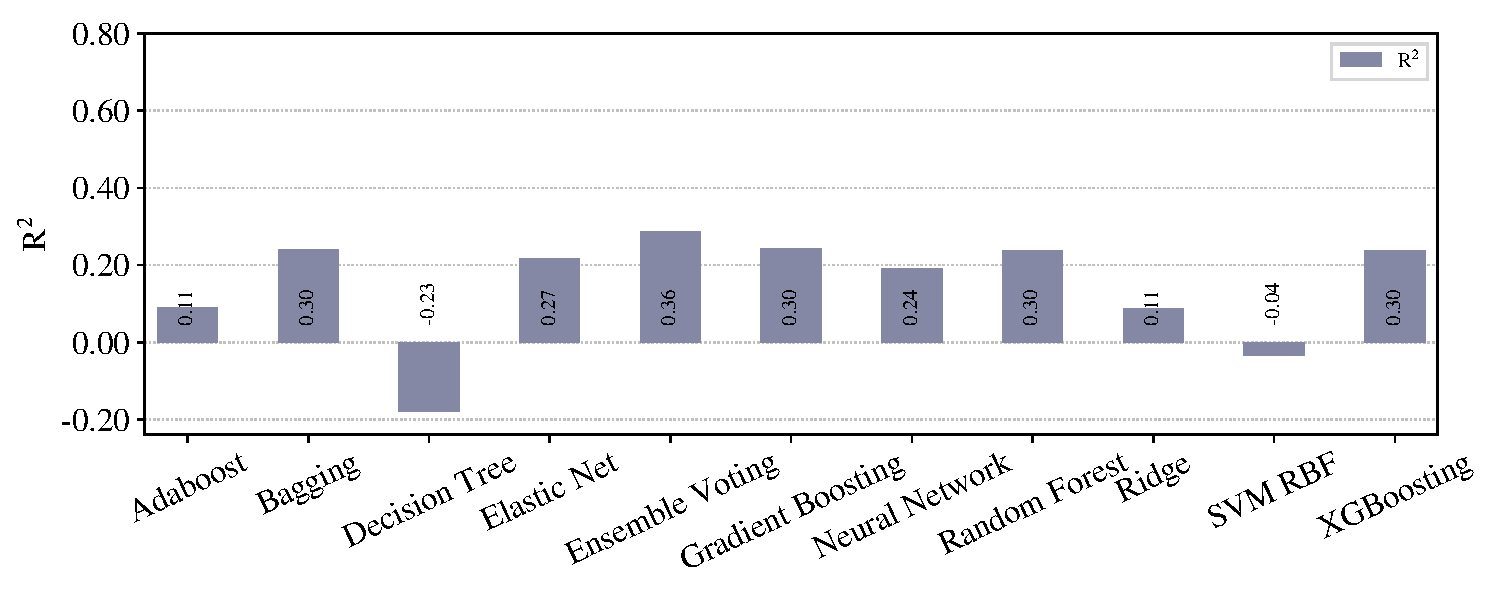
\includegraphics[width=\textwidth]{images/chapters/results_regression_all_off_r2.pdf}
\end{figure}

\begin{figure}[!htb]
  \centering
  \caption{Results for MAE and RMSE from baseline pipeline}
  \label{fig:results_base_case_error}
  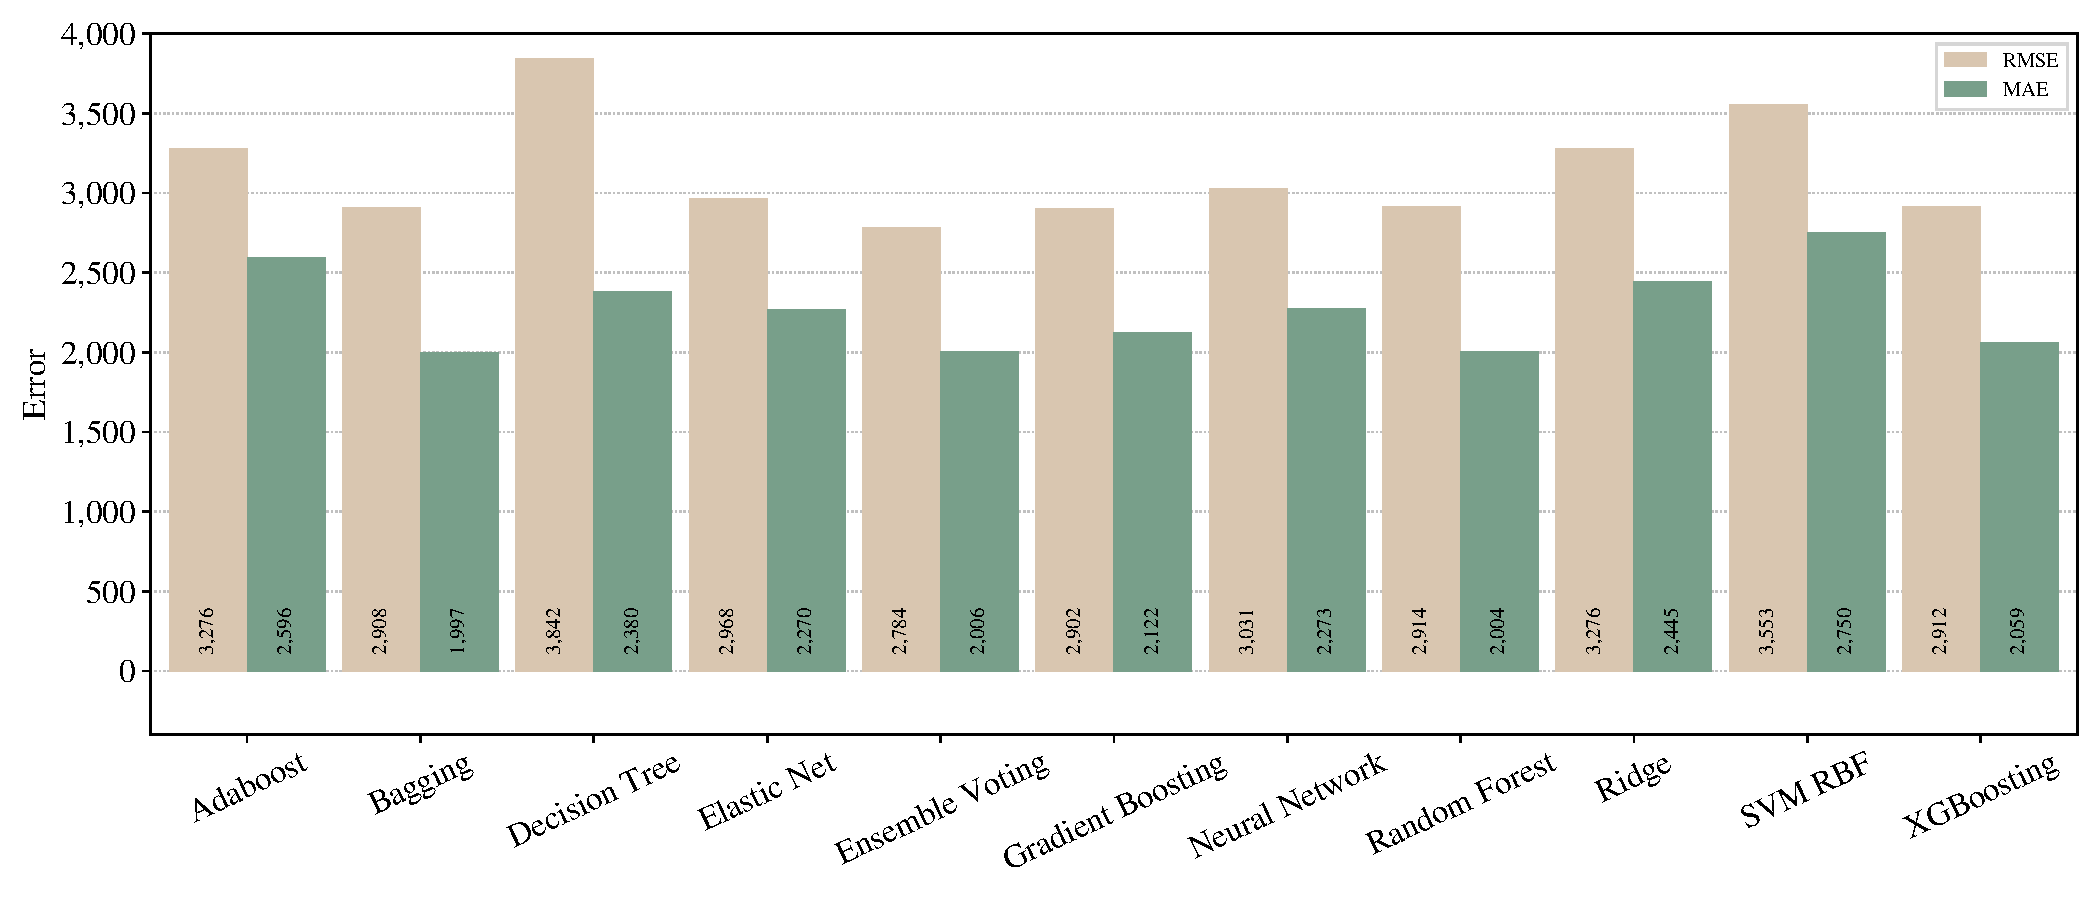
\includegraphics[width=\textwidth]{images/chapters/results_regression_all_off_mae_rmse_test.pdf}
\end{figure}

We repeated the steps from Section \ref{sec:regression_pipeline} for the \textit{full} pipeline with all adjustments activated (except outliers removal in training data) and the achieved results are shown in Figure \ref{fig:results_full_pipeline_r2} and Figure \ref{fig:results_full_pipeline_error}.

\begin{figure}[htb]
  \centering
  \caption{Results for R$^2$ from full pipeline}
  \label{fig:results_full_pipeline_r2}
  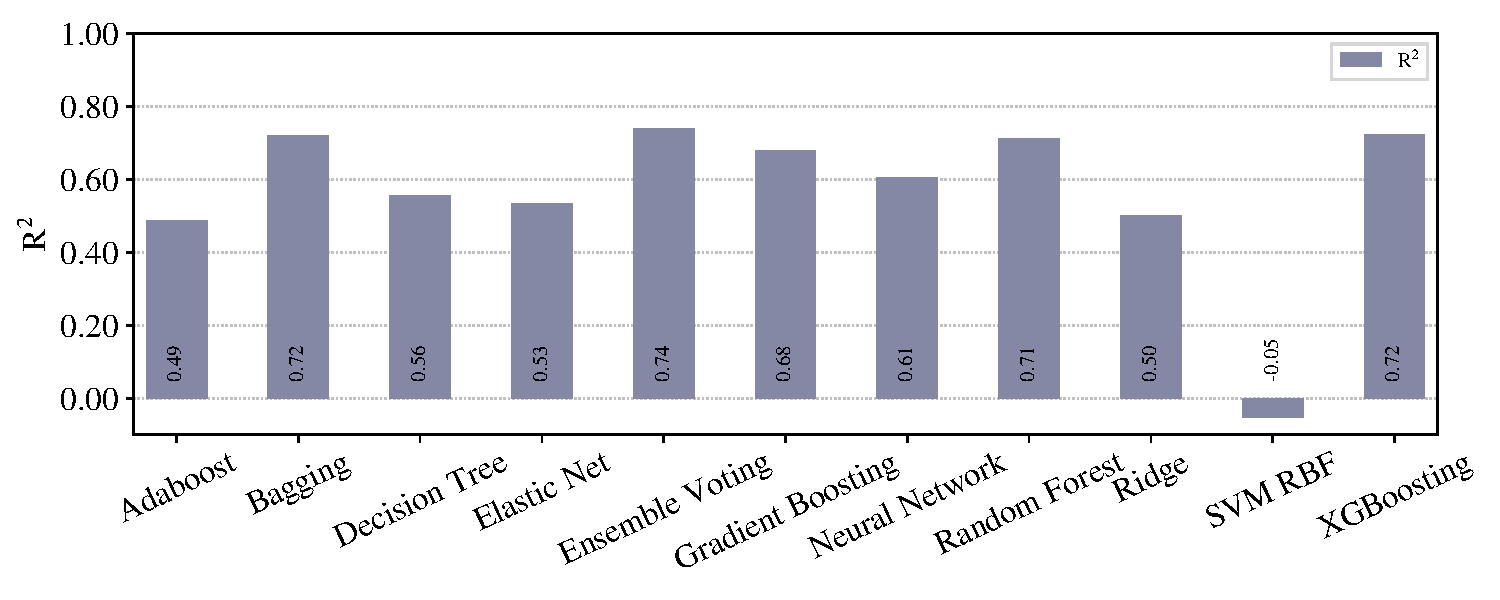
\includegraphics[width=\textwidth]{images/chapters/results_regression_all_set_r2.pdf}
\end{figure}

\begin{figure}[htb]
  \centering
  \caption{Results for MAE and RMSE from full pipeline}
  \label{fig:results_full_pipeline_error}
  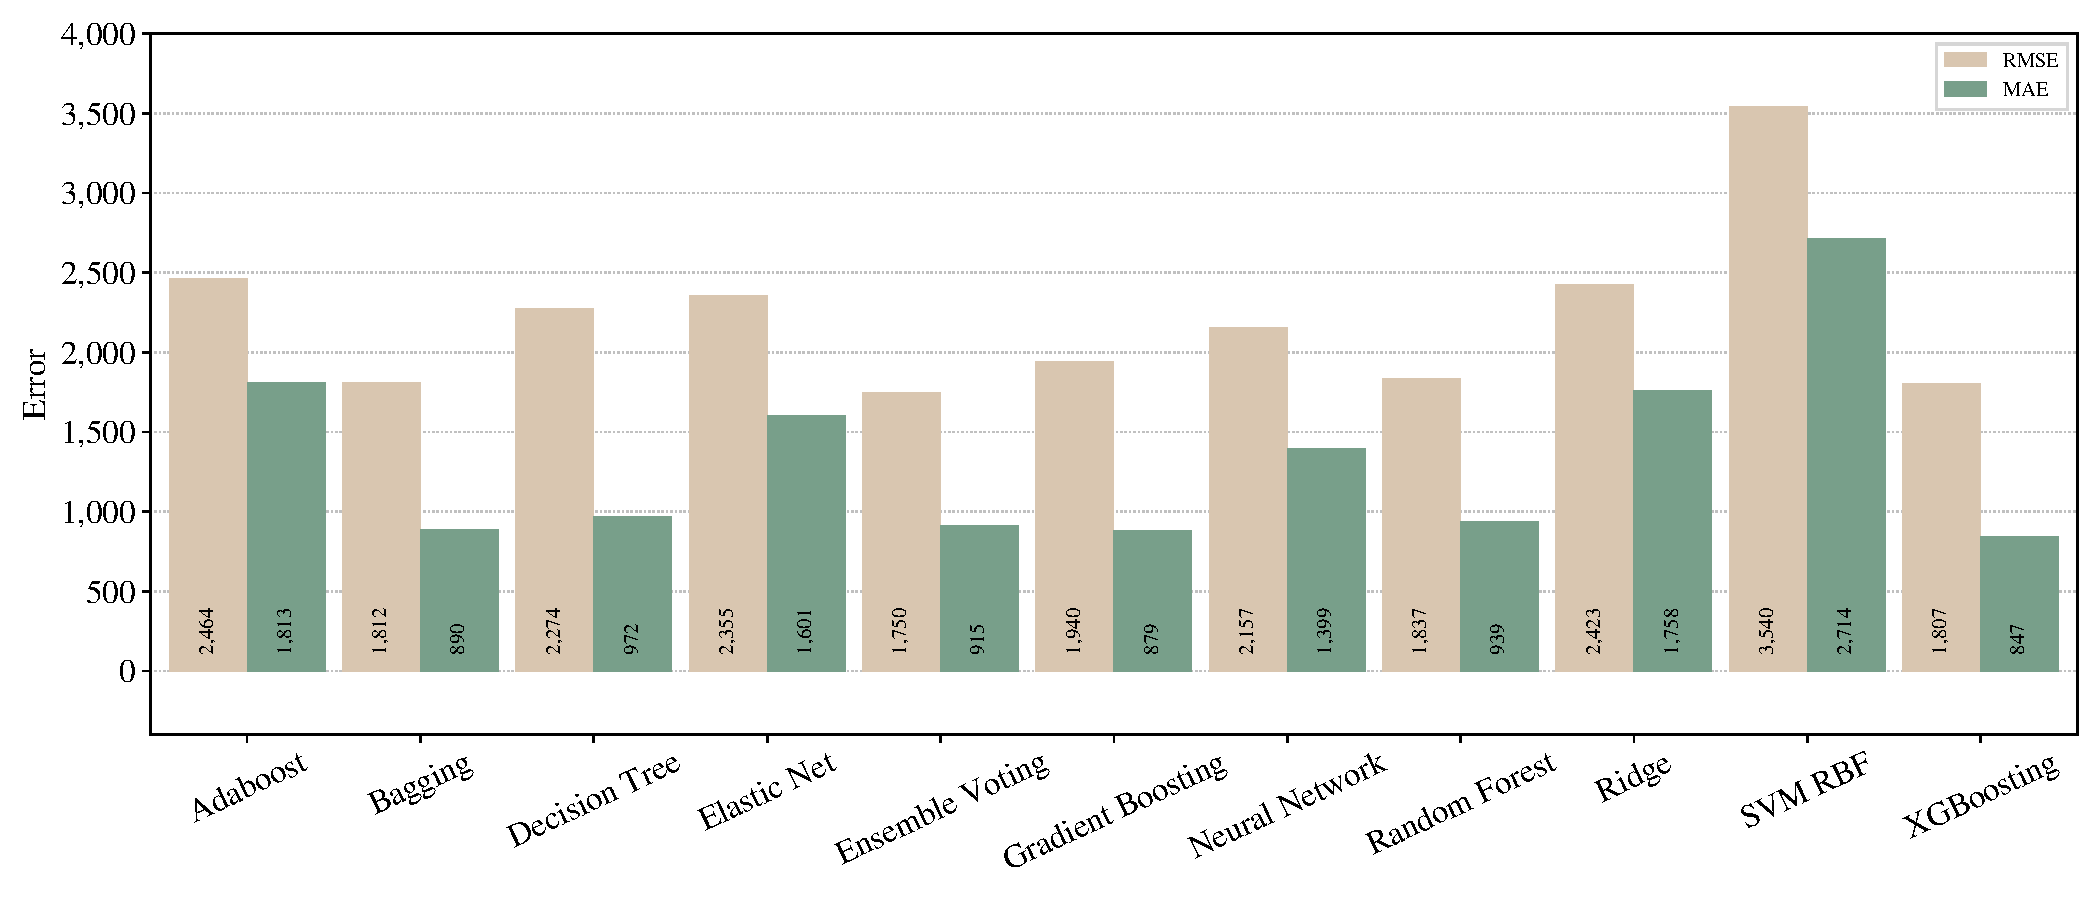
\includegraphics[width=\textwidth]{images/chapters/results_regression_all_set_mae_rmse_test.pdf}
\end{figure}

From Figures \ref{fig:results_base_case_r2}, \ref{fig:results_base_case_error}, \ref{fig:results_full_pipeline_r2}, and \ref{fig:results_full_pipeline_error}, one can note significant improvements on the three metrics for most of the techniques, when we compare the \textit{baseline} and \textit{full} pipeline. The exception is \gls{SVM} with \gls{RBF} kernel. In that case, we can affirm that \gls{SVM} is underfitted, as the poor results stood regardless the pipelines we would apply. On the other hand, in terms of the best techniques, we can realize that Ensemble Voting achieved the best results among the techniques in terms of \gls{RMSE} and R$^2$. Thus, merging the techniques in Ensemble Voting achieved better results when compared to the models alone for R$^2$ and \gls{RMSE}. XGBoosting achieved the best prediction quality in terms of \gls{MAE}. 

% TODO: check this affirmation in Background
% As described in Chapter~\ref{cap:ml_text}, \gls{RMSE} tends to penalize bigger errors, so we can state that Ensemble Voting has fewer large errors than XGBoosting. Still, it predicts incorrectly more examples than XGBoosting.

As expected, we can conclude that the \textit{full} pipeline leads to better results than \textit{baseline}. Moreover, from the legal expert experience, a \gls{MAE} of less than 1,000 can be considered almost irrelevant in the context of legal compensation. 


\subsubsection{Results from combinations of adjustments}

This section shows the performance of combinations of adjustments and whether they achieved any better result when compared to the \textit{full} pipeline. Considering again Figure \ref{fig:pipeline}, we randomly selected a total of eighty different pipelines. 
%
When an adjustment is deactivated, its predecessor step in the pipeline is connected to its successor. For example, if we deactivate \textit{N-Grams Extraction}, the preprocessing step will be connected to the representation step and so on. 
%
Furthermore, the pipeline stays the same despite the (de)activation of \textit{Overfitting Avoidance} adjustment. This adjustment is more related to the configuration for the training step, that is, use complex (when deactivated) or simpler models (when activated) from Table \ref{tab:models}.

We represent a combination of adjustments as a binary number. If the adjustment is deactivated the digit is zero, and it is one otherwise. We assigned the positions to adjustments in the binary number in this order, from left to right: \textit{Feature Selection}, \textit{Outliers Removal (Train Set)}, \textit{N-Grams Extraction}, \textit{Addition of \gls{AELE}}, \textit{Cross-Validation}, \textit{Overfitting Avoidance} and \textit{Outliers Removal (All Dataset)}.

Figure \ref{fig:combinations_r2} shows the results, in which the $x$-axis represents the combinations, the $y$-axis represents the R$^2$ metric and each line is a different technique. To better detect the patterns, we have arranged the combinations in decreasing order of R$^2$ from Ensemble Voting regression. Following the same idea, Figure \ref{fig:combinations_rmse} shows the results for \gls{RMSE} with the same order of combinations in the $x$-axis.


% Tabela com as combinações e explicação que encontramos um melhor caso que não inclui todos os nossos ajustes.

\begin{figure}[htb]
  \centering
  \caption{R$^2$ for the pipelines based on combinations of adjustments}
  \label{fig:combinations_r2}
  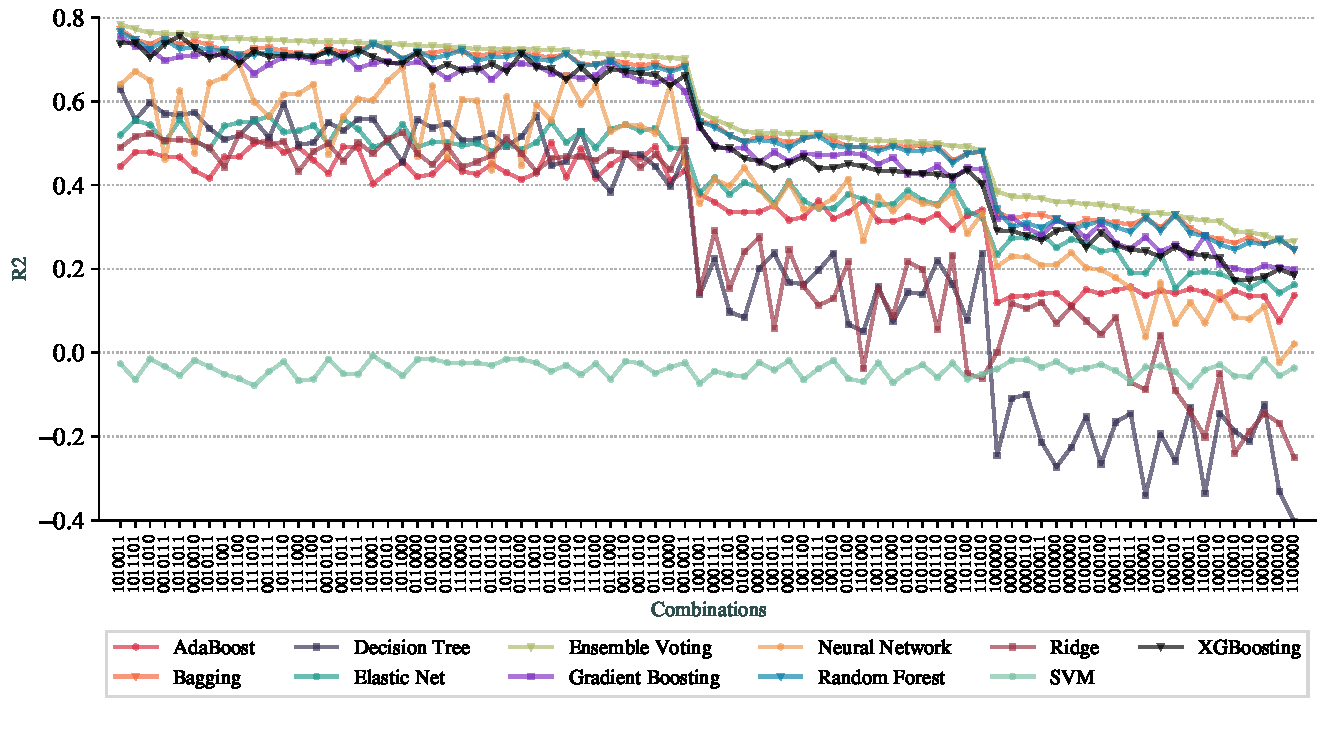
\includegraphics[width=\textwidth]{images/chapters/combinations_r2.pdf}
\end{figure}



\begin{figure}[htb]
  \centering
  \caption{RMSE for the pipelines based on combinations of adjustments}
  \label{fig:combinations_rmse}
  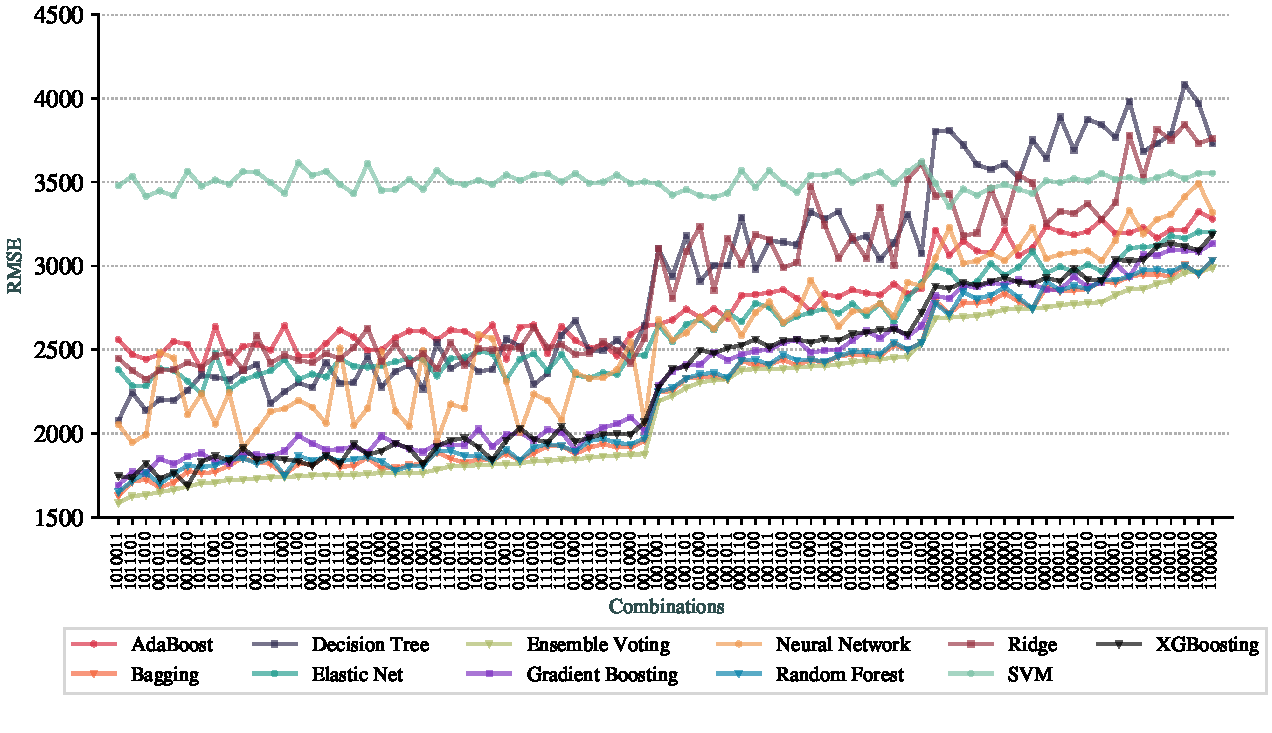
\includegraphics[width=\textwidth]{images/chapters/combinations_rmse.pdf}
\end{figure}


The first observation is that we can achieve prediction qualities better than the \textit{full} pipeline. The best pipeline, based on \gls{RMSE} and R$^2$, is represented as $1010011$, with \textit{Feature Selection}, \textit{N-Grams Extraction}, \textit{Overfitting Avoidance} and \textit{Outliers Removal (All Dataset)} activated while \textit{Outliers Removal (Train Set)}, \textit{Addition of \gls{AELE}} and \textit{Cross-Validation} deactivated. The best technique is the Ensemble Voting with R$^2$ of 0.78, \gls{RMSE} of 1,586 and \gls{MAE} of 803. The results for combinations for \gls{MAE} are not included due to the similarity to \gls{RMSE} results in terms of best and worst techniques.

We can observe that Ensemble Voting, Bagging, Random Forest, Gradient Boosting, and XGBoosting have the best result metrics as they stand at the top of the charts for most combinations. As worse technique, we have SVM, that performed poorer than other techniques in most combinations. Another observation is that the \textit{baseline} pipeline is better than 20 combinations in terms of prediction quality. That is, in terms of prediction quality, the pipeline without any \textit{adjustments} has better results than other pipelines that have some of them.

From a more global analysis of Figures \ref{fig:combinations_r2} and \ref{fig:combinations_rmse}, there are two sudden changes in the prediction quality. The first happens in the middle of the graphs for \gls{RMSE} and R$^2$ and the second appears in the third quarter. One can notice that most of the techniques exhibit this behavior of sudden change. The first change happens when the combinations no longer contain \textit{N-Grams Extraction} (third digit in the combinations) as, before that point, all combination had this adjustment. We can also note that \textit{Addition of \gls{AELE}} (fourth digit in the combinations) starts to appear consistently in all combinations from this point. 

The second sudden change happens when \textit{Addition of \gls{AELE}} stops appearing in the combinations. As we described, the best combination does not have this adjustment, but at this point, it has such an impact on the prediction quality. Thus, we can point the cause of this difference to the presence of \textit{N-Grams Extraction}. When N-Grams is activated, the impact of \textit{Addition of \gls{AELE}} on the prediction quality is reduced and it increases in the combinations without \textit{N-Grams Extraction}. This pattern is shared among all models except \gls{SVM}, which did not perform well in any combinations.

Although different combinations of adjustments can lead to results better than the full pipeline, 
it is important to quantify how much each adjustment impacts the results. As demonstrated, \textit{N-Grams Extraction} and \textit{Addition of \gls{AELE}} have a considerable impact on the prediction quality.


%%%%%%%%%%%%%%%%%%%%%%%%%%%%%%%%%%%%%%%%%%%%%%%%%%%%%%%%%%%%%%%%%%
\subsubsection{Impact of each adjustment on the performance}

This section discusses how each adjustment impacts the prediction quality and execution time (total time to run a pipeline). We investigate how much \gls{RMSE}, R$^2$, and execution time increase or decrease as we add or remove steps in the pipeline. To do so, we consider all the eighty combinations of pipelines we have tested, and an adjustment we want to evaluate. First, we select the combination with an adjustment bypassed, which is compared directly to the corresponding combination with the same adjustment activated.

Then, for each pair, we take the difference of the metrics. Finally, to estimate the overall influence of the adjustment on the results, the average plus/minus the standard deviation of the differences is considered. By doing this, we can determine how much a specific adjustment influences the results since it is the only difference.
% Show the results
Table \ref{tab:impact_rmse} contains the results for \gls{RMSE} and Table \ref{tab:impact_r2} the results for R$^2$. 

Each value represents the average plus/minus standard deviation of how much the adjustment increased/decreased the metric in the technique. We also highlighted the values in which the adjustment has its biggest impact. For instance, in average, including the \textit{Addition of \gls{AELE}} decreased the \gls{RMSE} in $304 \pm 365$ in Decision Trees. We can notice that the impact can have a significant variance according to the combinations, since standard deviation shows how much the adjustments can \textit{influence} each other's impacts.

%%%%%% RMSE Impact $$$$$$$$$$$
\begin{table}[htb]
  \setlength{\tabcolsep}{4.0pt}
 \caption{Impact of adjustments on RMSE}
 \label{tab:impact_rmse}

\footnotesize
\begin{tabular}{crrrrrrr}
\hline
\textbf{Technique} & \multicolumn{1}{c}{\textbf{\begin{tabular}[c]{@{}c@{}}Feature\\ Selection\end{tabular}}} & \multicolumn{1}{c}{\textbf{\begin{tabular}[c]{@{}c@{}}Addittion\\ of\\AELE\end{tabular}}} & \multicolumn{1}{c}{\textbf{\begin{tabular}[c]{@{}c@{}}Cross-\\ Validation\end{tabular}}} & \multicolumn{1}{c}{\textbf{\begin{tabular}[c]{@{}c@{}}N-Grams\\ Extraction\end{tabular}}} & \multicolumn{1}{c}{\textbf{\begin{tabular}[c]{@{}c@{}}Overfitting\\ Avoidance\end{tabular}}} & \multicolumn{1}{c}{\textbf{\begin{tabular}[c]{@{}c@{}}Outliers\\ Removal\\ (Train)\end{tabular}}} & \multicolumn{1}{c}{\textbf{\begin{tabular}[c]{@{}c@{}}Outliers\\ Removal\\ (All Dataset)\end{tabular}}} \\ \hline
AB      & 4 $\pm~$61                                          & -250 $\pm~$149               & 6 $\pm~$52                                          & -447 $\pm~$161              & -21 $\pm~$56                                           & -\textbf{35 $\pm~$48}                                             & -93 $\pm~$83                                                \\
BG      & 12 $\pm~$99                                         & -219 $\pm~$255               & 6 $\pm~$80                                          & -816 $\pm~$258              & 0 $\pm~$78                                            & 20 $\pm~$82                                              & -104 $\pm~$96                                                \\
DT   & -40 $\pm~$156                                        & \textbf{-304 $\pm~$365}               & 18 $\pm~$111                                         & \textbf{-1078 $\pm~$359}             & \textbf{-168 $\pm~$107}                                         & 47 $\pm~$107                                             & -90 $\pm~$139                                                \\
EN    & 75 $\pm~$78                                         & -222 $\pm~$124               & 15 $\pm~$64                                         & -493 $\pm~$139              & 8 $\pm~$65                                            & 25 $\pm~$56                                              & -54 $\pm~$61                                                \\
EV  & 17 $\pm~$107                                         & -222 $\pm~$228               & 11 $\pm~$84                                         & -829 $\pm~$229              & 7 $\pm~$88                                            & 31 $\pm~$84                                              & -93 $\pm~$95                                                \\
GB & 9 $\pm~$129                                         & -236 $\pm~$244               & 17 $\pm~$88                                         & -811 $\pm~$240              & 39 $\pm~$107                                           & 43 $\pm~$100                                             & -86 $\pm~$115                                                \\
NN   & \textbf{-57 $\pm~$255}                                        & -279 $\pm~$210               & 5 $\pm~$95                                          & -742 $\pm~$316              & 21 $\pm~$119                                           & 87 $\pm~$98                                              & -31 $\pm~$104                                                \\
RF   & 9 $\pm~$95                                          & -220 $\pm~$257               & 5 $\pm~$79                                          & -811 $\pm~$260              & 28 $\pm~$74                                           & 15 $\pm~$81                                              & -108 $\pm~$91                                                \\
RG       & 206 $\pm~$209                                        & -181 $\pm~$188               & \textbf{-23 $\pm~$99}                                         & -860 $\pm~$249              & -1 $\pm~$105                                           & 125 $\pm~$125                                             & -52 $\pm~$98                                                \\
\gls{SVM} RBF      & 21 $\pm~$47                                         & 33 $\pm~$54                 & 10 $\pm~$42                                         & 11 $\pm~$57               & -10 $\pm~$56                                           & 30 $\pm~$58                                              & -32 $\pm~$65                                                \\
XGB     & 37 $\pm~$119                                         & -244 $\pm~$234               & 8 $\pm~$84                                          & -873 $\pm~$233              & 27 $\pm~$99                                           & 29 $\pm~$81                                              & \textbf{-117 $\pm~$101}   \\ \hline
\end{tabular}

 %{\begin{tabnote}
 %Source:
 %\end{tabnote}}
\end{table}

%%%%%%% R2 Imapct #############
\begin{table}[htb]

\footnotesize
\setlength{\tabcolsep}{3pt}
 \caption{Impact of adjustments on R$^2$}
 
 \label{tab:impact_r2}
\begin{tabular}{crrrrrrr}
\hline
\textbf{Technique} & \multicolumn{1}{c}{\textbf{\begin{tabular}[c]{@{}c@{}}Feature\\ Selection\end{tabular}}} & \multicolumn{1}{c}{\textbf{\begin{tabular}[c]{@{}c@{}}Addition of\\ AELE\end{tabular}}} & \multicolumn{1}{c}{\textbf{\begin{tabular}[c]{@{}c@{}}Cross-\\ Validation\end{tabular}}} & \multicolumn{1}{c}{\textbf{\begin{tabular}[c]{@{}c@{}}N-Grams\\ Extraction\end{tabular}}} & \multicolumn{1}{c}{\textbf{\begin{tabular}[c]{@{}c@{}}Overfitting\\ Avoidance\end{tabular}}} & \multicolumn{1}{c}{\textbf{\begin{tabular}[c]{@{}c@{}}Outliers\\ Removal\\ (Train)\end{tabular}}} & \multicolumn{1}{c}{\textbf{\begin{tabular}[c]{@{}c@{}}Outliers\\ Removal\\ (All Dataset)\end{tabular}}} \\ \hline
AB      & 0.00 $\pm~$0.02                                       & 0.12 $\pm~$0.08               & 0.00 $\pm~$0.02                                       & 0.22 $\pm~$0.08             & 0.01 $\pm~$0.02                                         & \textbf{0.02 $\pm~$0.02}                                            & 0.02 $\pm~$0.02                                               \\
BG      & -0.01 $\pm~$0.03                                       & 0.10 $\pm~$0.11               & 0.00 $\pm~$0.02                                       & 0.32 $\pm~$0.11             & 0.00 $\pm~$0.02                                         & -0.01 $\pm~$0.03                                           & 0.02 $\pm~$0.03                                               \\
DT   &\textbf{ 0.02 $\pm~$0.07}                                       & \textbf{0.18 $\pm~$0.20}               & -0.01 $\pm~$0.05                                       & \textbf{0.55 $\pm~$0.20}            & \textbf{0.09 $\pm~$0.06}                                         & -0.03 $\pm~$0.05                                           & 0.01 $\pm~$0.07                                               \\
EN    & -0.03 $\pm~$0.04                                       & 0.10 $\pm~$0.06               & -0.01 $\pm~$0.02                                       & 0.23 $\pm~$0.07             & 0.00 $\pm~$0.02                                         & -0.01 $\pm~$0.02                                           & 0.00 $\pm~$0.02                                               \\
EV  & -0.01 $\pm~$0.04                                       & 0.10 $\pm~$0.10               & 0.00 $\pm~$0.03                                       & 0.31 $\pm~$0.10             & 0.00 $\pm~$0.03                                         & -0.01 $\pm~$0.03                                           & 0.02 $\pm~$0.03                                               \\
GB & -0.01 $\pm~$0.05                                       & 0.11 $\pm~$0.11               & -0.01 $\pm~$0.03                                       & 0.33 $\pm~$0.11             & -0.02 $\pm~$0.04                                         & -0.02 $\pm~$0.04                                           & 0.01 $\pm~$0.04                                               \\
NN   & 0.01 $\pm~$0.11                                       & 0.14 $\pm~$0.11               & 0.00 $\pm~$0.04                                       & 0.34 $\pm~$0.15             & 0.00 $\pm~$0.06                                         & -0.04 $\pm~$0.04                                           & -0.01 $\pm~$0.05                                              \\
RF   & -0.01 $\pm~$0.03                                       & 0.10 $\pm~$0.11               & 0.00 $\pm~$0.02                                       & 0.32 $\pm~$0.11             & -0.01 $\pm~$0.02                                         & -0.01 $\pm~$0.03                                           & 0.02 $\pm~$0.03                                               \\
RG       & -0.11 $\pm~$0.12                                       & 0.10 $\pm~$0.10               & \textbf{0.01 $\pm~$0.05}                                       & 0.44 $\pm~$0.14             & 0.00 $\pm~$0.05                                         & -0.07 $\pm~$0.07                                           & 0.00 $\pm~$0.04                                               \\
\gls{SVM} RBF      & -0.01 $\pm~$0.01                                       & -0.02 $\pm~$0.02              & 0.00 $\pm~$0.01                                       & 0.01 $\pm~$0.02             & 0.01 $\pm~$0.02                                         & -0.01 $\pm~$0.02                                           & -0.01 $\pm~$0.02                                              \\
XGB     & -0.02 $\pm~$0.04                                       & 0.11 $\pm~$0.11               & 0.00 $\pm~$0.03                                       & 0.35 $\pm~$0.11             & -0.01 $\pm~$0.04                                         & -0.01 $\pm~$0.03                                           & \textbf{0.03 $\pm~$0.04}                                               \\ \hline
\end{tabular}
% \begin{tabular}{@{}cccccccc@{}}
% \toprule
% \textbf{Technique}          & \textbf{\begin{tabular}[c]{@{}c@{}}Feature\\ Selection\end{tabular}} & \textbf{Attributes} & \textbf{\begin{tabular}[c]{@{}c@{}}Cross-\\ Validation\end{tabular}} & \textbf{N-Grams} & \textbf{\begin{tabular}[c]{@{}c@{}}Overfitting\\ Avoidance\end{tabular}} & \textbf{\begin{tabular}[c]{@{}c@{}}Outliers\\ Removal\\ (Train Set)\end{tabular}} & \textbf{\begin{tabular}[c]{@{}c@{}}Outliers\\ Removal\\ (Dataset)\end{tabular}} \\ \midrule
% Adaboost              & 0,00    & 0,12    & 0,00    & 0,22    & 0,01    & \textbf{0,02}     & 0,02     \\
% Bagging              & -0,01    & 0,10    & 0,00    & 0,32    & 0,00    & -0,01    & 0,02     \\
% Decision Tree           & \textbf{0,02}    & \textbf{0,18}    & -0,01    & \textbf{0,55}    & \textbf{0,09}    & -0,03    & 0,01     \\
% Elastic Net            & -0,03    & 0,10    & -0,01    & 0,23    & 0,00    & -0,01    & 0,00     \\
% Ensemble Voting & -0,01    & 0,10    & 0,00    & 0,31    & 0,00    & -0,01    & 0,02     \\
% Gradient Boosting         & -0,01    & 0,11    & -0,01    & 0,33    & -0,02    & -0,02    & 0,01     \\
% Neural Network               & 0,01    & 0,14    & 0,00    & 0,34    & 0,00    & -0,04    & -0,01    \\
% Random Forest           & -0,01    & 0,10    & 0,00    & 0,32    & -0,01    & -0,01    & 0,02     \\
% Ridge               & -0,11    & 0,10    & \textbf{0,01}    & 0,44    & 0,00    & -0,07    & 0,00     \\
% \gls{SVM}           & -0,01    & -0,02    & 0,00    & 0,01    & 0,01    & -0,01    & -0,01    \\
% XGBoosting              & -0,02    & 0,11    & 0,00    & 0,35    & -0,01    & -0,01    & \textbf{0,03 }    \\ \bottomrule
% \end{tabular}

%  {\begin{tabnote}
%  %Source:
%  \end{tabnote}}
\end{table}



% Interpret the results.
From Tables \ref{tab:impact_rmse} and \ref{tab:impact_r2}, we confirm the observations from the previous sections about the sudden changes in which the combinations stopped to have \textit {N-Grams Extraction} or \textit{Addition of \gls{AELE}}. Here, we measure the impact of these two adjustments and their impact on the prediction quality.

In terms of techniques, the adjustments have more significant impact on the Decision Tree and least impact on \gls{SVM}. Tree-based methods, such as XGBoosting, Random Forest and Bagging, also performed significantly better with the application of the adjustments. 
% Evaluate Feature Selection
Tables \ref{tab:impact_rmse} and \ref{tab:impact_r2} also show that \textit{Feature Selection} has a small negative impact.

Regarding the \emph{execution time}, Table \ref{tab:execution_time} contains the results. It presents the average execution time plus/minus standard deviation of the whole pipeline. The value is based on the ratio between the execution time when the adjustment is activated and when it is bypassed. Thus, if we have a positive percentage, the activated adjustment increases the execution time, and it decreases when the percentage is negative. We do not show absolute values of time due to the differences in the available computer power in the market. 

\begin{table}[htb]

\footnotesize
  \setlength{\tabcolsep}{4pt}
\caption{Percentage impact of adjustments on execution time}
\label{tab:execution_time}
\begin{tabular}{@{}ccccccc@{}}
\toprule
\textbf{\begin{tabular}[c]{@{}c@{}}Feature\\ Selection\end{tabular}} & \textbf{\begin{tabular}[c]{@{}c@{}}Addition of\\ AELE\end{tabular}}      & \textbf{\begin{tabular}[c]{@{}c@{}}Cross-\\ Validation\end{tabular}} & \textbf{\begin{tabular}[c]{@{}c@{}}N-Grams\\ Extraction\end{tabular}}        & \textbf{\begin{tabular}[c]{@{}c@{}}Overfitting\\ Avoidance\end{tabular}} & \textbf{\begin{tabular}[c]{@{}c@{}}Outliers\\ Removal\\ (Train)\end{tabular}} & \textbf{\begin{tabular}[c]{@{}c@{}}Outliers\\ Removal\\ (All Dataset)\end{tabular}} \\ \midrule
\multicolumn{1}{c}{-91.7\% $\pm~$5.0}                   & \multicolumn{1}{c}{48.1\% $\pm~$35.6} & \multicolumn{1}{c}{371.4\% $\pm~$49.5}                   & \multicolumn{1}{c}{29.6\% $\pm~$30.7} & \multicolumn{1}{c}{-75.8\% $\pm~$11.9}                     & \multicolumn{1}{c}{-10.8\% $\pm~$5.5}                        & \multicolumn{1}{c}{-11.0\% $\pm~$5.5}                           \\ \bottomrule
\end{tabular}

						

%  {\begin{tabnote}
%  %Source:
%  \end{tabnote}}
\end{table}


% Overfitting Avoidance
Even though \textit{Feature Selection} leads to worse results, when it is activated, the execution time decreases by more than ninety per cent. Something similar happens to \textit{Overfitting Avoidance} since it also has little impact, but the execution time reduces by more than seventy five per cent. Therefore, there is a trade-off between execution time and prediction quality we have to choose. It pays off to have \textit{Feature Selection} and \textit{Overfitting Avoidance} adjustments in our pipeline, since when we have both bypassed executing the whole pipeline took hours in our experiments, while it took minutes in the opposite situation. Reducing the sizes of the input and the models also reduce the execution time.

% Cross-validation
Although we can see that \textit{Cross-Validation} also has little impact on the prediction quality in the regression task, it increases the execution time almost five times. As presented in Section \ref{sec:basic_definitions}, cross-validation tends to produce results with less bias since it generates five different combinations to train and test our models. But, in this case, we do not see this effect. The twenty five repetitions we run without \textit{Cross-Validation} produced different combinations of train and test sets with a good amount of variability to capture a good estimate of the model's prediction quality. Thus, the five-fold extra combinations from cross-validation do not impact the results significantly in our experiments. Except for the time execution, which took almost five times longer.

% Outlier Removal
\textit{Outliers Removal} also do not impact significantly the results. But we can see that the two approaches, that is, removing outliers in the train data or the whole dataset, influence the results in different ways. While the former tends to lead to worse results, the latter leads to better results. When we remove outliers from train data and keep them in the test data, the models make poor predictions for the outliers but, if we keep our entire dataset away from anomalies, the models get better prediction quality results.

% Talk again about N-grams and attributes regarding time execution.
We also note that \textit{N-Grams Extraction} and \textit{Addition of \gls{AELE}}, in terms of execution time, tend to impact negatively the pipeline, as shown in Table \ref{tab:execution_time}. Still, the improvement in the pipeline results overlaps this additional execution time when considering the high gains in prediction quality on adding these adjustments.


Considering prediction quality and execution time, the best combination is $1011011$, with the adjustments \textit{Feature Selection}, \textit{N-Grams Extraction}, \textit{Addition of \gls{AELE}}, \textit{Overfitting Avoidance} and \textit{Outliers Removal} from all dataset activated and the remaining deactivated. This is the fifth combination from Figures \ref{fig:combinations_r2} and \ref{fig:combinations_rmse}. In terms of prediction quality, the best models are Ensemble Voting and XGBoosting, where the former has a \gls{RMSE} of 1,684, a \gls{MAE} of 866 and R$^2$ of 0.76, and the latter has a \gls{RMSE} of 1,689, a \gls{MAE} of 792 and R$^2$ of 0.76, as shown in Figure \ref{fig:results_best_pipeline_r2} and Figure \ref{fig:results_best_pipeline_error}.

% Colocar figura aqui.
% TODO: Checar aqui
\begin{figure}[!htb]
  \centering
  \caption{Results for R$^2$ from the best pipeline}
  \label{fig:results_best_pipeline_r2}
  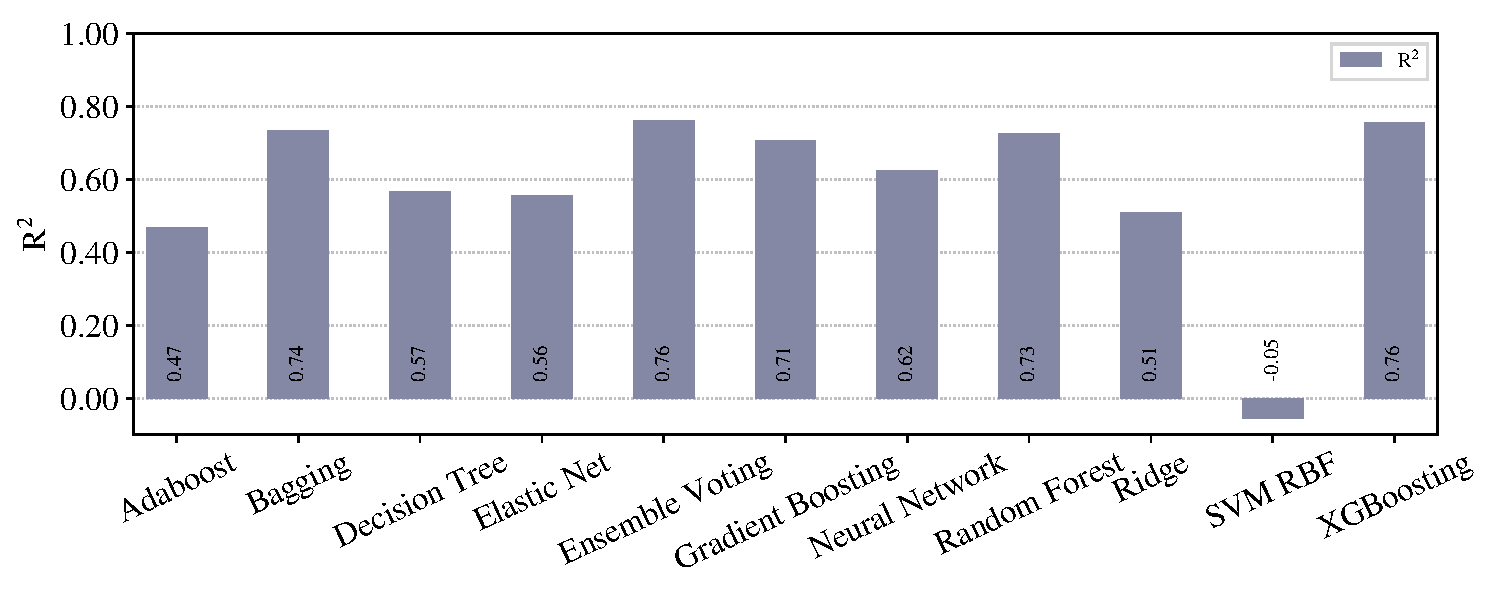
\includegraphics[width=\textwidth]{images/chapters/results_regression_best_r2.pdf}
\end{figure}

\begin{figure}[!htb]
  \centering
  \caption{Results for MAE and RMSE from the best pipeline}
  \label{fig:results_best_pipeline_error}
  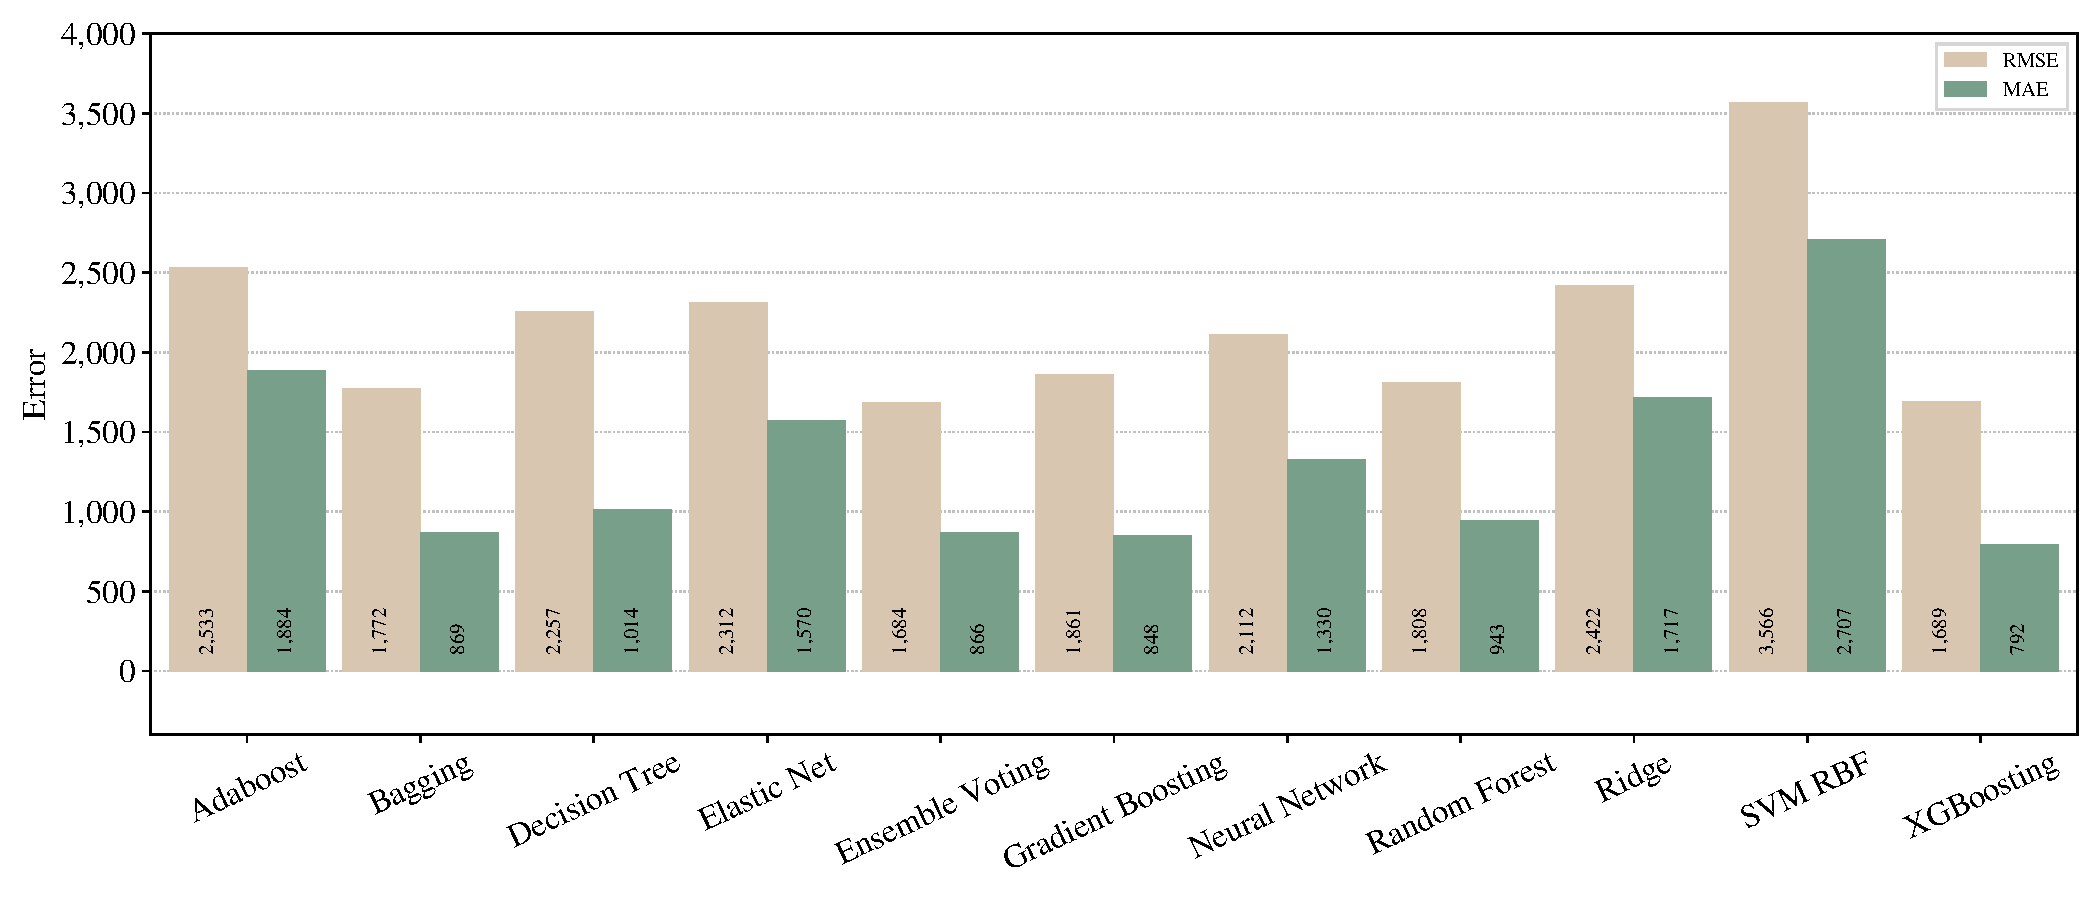
\includegraphics[width=\textwidth]{images/chapters/results_regression_best_mae_rmse.pdf}
\end{figure}
%To what extent the prediction of compensation values can be \emph{accurate} and \emph{helpful} in the legal environment using regression models?

Finally, recalling the research question and based on the discussion above, the prediction of compensation can be \textit{accurate} by using the combination $1011011$, when \textit{Feature Selection}, \textit{N-Grams Extraction}, \textit{Addition of \gls{AELE}}, \textit{Overfitting Avoidance} and \textit{Outliers Removal} from all dataset are activated and the remaining deactivated. 
Based on the evaluation of the results, the legal expert's experience shows that the predictions are \textit{helpful} in the legal environment and can encourage the parties involved (consumer and airline) in an agreement. The \gls{MAE} error of the best pipeline was 792.00. That way, giving up approximately 1,000 Brazilian Reais of the compensation is acceptable in conciliation hearings (an initial lawsuit stage in which the parties try to negotiate to solve the case themselves). For example, the consumer who will earn R\$ 5,000 only at the end of the lawsuit, will agree more easily to being compensated in R\$ 4,000 in the beginning, so the case is closed immediately.



